\chapter{What is policy-agnostic programming?\label{chap:PAP}}

Before we talk about policy-agnostic programming, we first need to give an
introduction to the domain it belongs to, i.e. information flow security.

\section{A brief overview of information flow security}

Information flow security is a security mechanism that consists of information flow
policies and information flow controls to detect and prevent leaking of sensitive
data by an application. Information flow policies here are the policies that define
where sensitive data can flow. Information flow controls are the mechanisms that
enforce them.

\subsection{Basic principles of information flow security}
When designing a system with information flow security, sensitive data needs to
be identified and corresponding information flow policies need to be defined.
Smith~\cite{PrincInfoSec} talks about basic principles of information flow security
that we mention here in brief.
\subsubsection{Security labels}
We assign \textit{security} labels to variables
according to the level of security they are classified into. The most basic labels
are L for low security or public information and H for high security or private
information; goal is to prevent improper leaks of information in H variables to
L variables. The flow of data from an L variable into an H variable is legal.

\subsubsection{Explicit and implicit flow}
In information flow security, the leak can be in terms of an \textit{explicit flow}
or an \textit{implicit flow}. The following is an example of an \textit{explicit flow} where there is a direct
flow of data from an H variable to an L variable: \\
\indent
\texttt{public\textsubscript{L} = confidential\textsubscript{H}}
\eject
\noindent \\
The code-snippet below is an example of an \textit{implicit flow}: \\
\indent
	\texttt{if (confidential\textsubscript{H} \% 2)  == 0 \\ \indent \indent
		public\textsubscript{L} = 0 \\ \indent
	else \\ \indent \indent
		public\textsubscript{L} = 1} \\
\noindent Although it may not seem obvious that there is a leak of sensitive data
in this example, the last bit of the H variable (\texttt{confidential\textsubscript{H}})
is being copied into the L variable (\texttt{public\textsubscript{L}}). Any case
where there is a branching statement that depends on an H variable has a potential
data leak in terms of an \textit{implicit flow}.

\subsubsection{Noninterference \label{sec:noninterference}}
An important property in information flow security is noninterference. Smith~\cite{PrincInfoSec},
defines a program satisfying noninterference as:

\begin{quotation}
	\noindent Program $c$ satisfies noninterference if, for
	any memories $\mu$ and $v$ that agree on L variables, the memories produced by
	running $c$ on $\mu$ and on $v$ also agree on L variables (provided that both runs
	terminate successfully).
\end{quotation}
It is a formalization of the idea that a program should not leak
information about H (private) variables through L (public) variables. All systems
that provide information flow analysis need to prove noninterference. Although
strict noninterference is not desired since a real world system may need to change
labels or declassify (downgrade level of a variable) variables at runtime. One such
relaxed form of noninterference is \textit{termination-insensitive noninterference}
which still maintains the property of private inputs not influencing public outputs
on program execution although private information can influence the termination of
the program. Although the termination of a program is a publicly observable fact,
Austin and Flanagan~\cite{Faceted} found only one attack through this channel which
uses a brute force approach~\cite{TINI}.

\subsubsection{Confidentiality and integrity}
Information flow security is used to ensure \textit{confidentiality} and \textit{integrity}
of data. Our solution will mostly focus on \textit{confidentiality} but here we would
briefly like to define the two in the context of information flow security.
\textit{Confidentiality} as we have described above ensures that there is no unwanted
flow of information from H variables into L variables. For example, you wouldn't
want to allow the flow of data from a variable that contains credit card information
into a variable that is meant to store payment amount. \textit{Integrity} introduces
the concepts of tainted and untainted variables. Variables that contain information
received from an external source (network or user input) are marked as tainted. Here
the aim is to not allow the flow of information from tainted variables into untainted
variables. For example, data in a tainted variable needs to be sanitized before it
can be used as a parameter in an SQL query or as part of a string that is used as
input to the \texttt{eval} function. \texttt{eval} is a Javascript function that
takes Javascript code (in the form of a string) as input and executes it.

\subsection{Need for information flow security}
On the face of it information flow security may seem like an unnecessary overhead
for something that seems to have no real world use. This also seems to be the general
consensus since it has seen very little adoption in commercial software systems.
A majority of these systems rely on standard security mechanisms like access control,
encryption, and firewalls. Sabelfeld and Myers~\cite{LangInfo} show how these mechanisms
fall short in completely preventing sensitive data leaks. Access control is an
important part of any security infrastructure which is used to control access of
data to legitimate users but once access is granted, there is no way to control
how the data is used. Similarly, encryption will ensure that data will remain
confidential while in transit between two end-points but once the data is decrypted
at the receiving end, there is no way to control the flow of data from that point
onwards. A similar argument can be made for firewalls.

Yang~\cite{comey} in her blog post talks about a very popular privacy leak in recent
times. She explains how the leak was the result of a vulnerability that existed in
Instagram. While Instagram does protect the identity of users who wish to remain
private, it does not prevent their recommendation algorithms access to the same
data. The result of computations done by these algorithms is not protected which
is what led to the leak in this particular case.


\subsection{Language based information flow security \label{subsec:langinfo}}
There have been several approaches that researchers have tried to deal with the
problem of information flow security, primarily categorized into static and dynamic
analysis~\cite{Russo, Chlipala}. In recent years, a lot of the research has been
focussed on language-based approaches with the objective of making information
flow security a part of the programming language used for development. These are
mostly extensions to existing programming languages that provide constructs to define
labels, to specify policies, and to check those policies. As Sabelfeld and Myers~\cite{LangInfo}
discuss, the use of type systems for information flow analysis presents a promising
approach to get a practical implementation of information flow control. Here, every
expression has a security type with two parts: an ordinary type and a label that
describes how the value may be used. It is the job of the compiler to perform type
checking; whenever a program containing labelled types is read, the compiler also
makes sure that there will be no illegal flow of information at run-time. The authors
call such a type system that enforces information flow policies a \textit{security-type
system}.

Jif (Java + information flow) is an example of a language with a \textit{security-type system}
\cite{jifurl}, it extends Java with information flow controls and access controls
that are enforced at compile-time and run-time. It is based on the JFlow
language~\cite{Jflow}, which is the first usable programming model that provided
static information flow analysis.

The programming model introduced with Jif provides a robust set of features along
with the ability to specify information flow policies that are enforced by the Jif
compiler, but it is still not adopted in many practical, real-world systems. This
is largely due to the fact that a programmer must still have policy checking logic
all over the program whenever a sensitive value is used. When access to a sensitive
value is forbidden by a policy and the programmer has not handled such cases, the
program is likely to behave in an unexpected manner or get stuck. As Yang puts it
in her thesis~\cite{YangPhd}, handling all cases where sensitive variables are used
leads to ``programmer burden from policy spaghetti''. That is, using a system like
Jif results in policy checking logic scattered throughout the code. This leads to
code that is difficult to maintain and prone to human error. Another problem is
realized when these policies need to be changed, which would mean changes everywhere
the sensitive variable is used.

\section{The policy-agnostic programming model}
In an attempt to make the implementation of information flow security more flexible,
Yang et al~\cite{Jeeves} introduced the policy-agnostic programming (PAP) model.
PAP is an approach where the developer only needs to focus on writing core functionality
without the additional burden of thinking about data privacy constraints on sensitive
values.

PAP is introduced using Jeeves, a domain specific language that provides constructs
to define sensitive labels, policies, and to mark variables as sensitive. In
Jeeves, sensitive data has two views associated with it, a high confidentiality
view and a low confidentiality view. What view of the sensitive data is revealed
to a particular output channel depends on the ``context'' of the channel and the
policy associated with the sensitive data. ``Context'' here is an object that contains
relevant information that a policy may refer to. This can vary depending on the
application. Austin et al~\cite{FacetedJeeves} provide an example of a context
object for a health database application:\\
\indent \indent \texttt{HealthContext \{viewer: User, time: Date\}}\\
Here, the policies attached to sensitive variables will be resolved based on the
user who is trying to access a health record while time allows certain policies
to define expiration and activation times for visibility.
The goal of PAP is that you define all policies on sensitive variables when the
variables are defined. After this, everywhere the sensitive variables are used,
the language runtime is responsible for enforcing and checking the policies
associated with them.

The initial implementation of Jeeves involved symbolic evaluation and constraint
solving to produce outputs adhering to the policies associated with sensitive data.
This approach had limitations in terms of implementation feasibility and expressiveness,
which were later addressed by extending it with faceted values~\cite{FacetedJeeves}.
The faceted execution of policy-agnostic programs is based on work by Austin and
Flanagan~\cite{Faceted}.

\subsection{What is a faceted value?}
A faceted value as defined in~\cite{Faceted} is ``a triple consisting of a principal
$k$ and two values $V_H$ and $V_L$.'' It is represented as:
\[\langle k~?~V_H~:~V_L \rangle\]
Here you can imagine the principal $k$ to be the owner/guard of the sensitive value.
The faceted value appears as $V_H$ (private facet) to private observers that are
allowed to view $k$'s private data, and as $V_L$ (public facet) to other public
observers. In Jeeves, principals of faceted values have policies associated with
them which are rules that the ``guard'' will check before providing access to the
private facet. These policies need not be checked till the value needs to be revealed
to an output channel. So, while faceted values are flowing through a program, there
are special semantics that define how they should be evaluated. The following is
an example of a faceted value that specifies a sensitive email address:
\[\langle k~?~\text{`jon@sjsu.edu'}~:~\text{`[redacted]'} \rangle\]
When the policy associated with $k$ can be resolved to true, the value `jon@sjsu.edu'
is visible and if the policy is resolved to false, then the value `[redacted]' is
visible.

\subsection{Evaluation semantics of faceted values \label{sec:facetEval}}
The semantics of Jeeves are modeled using $\lambda^{jeeves}$ which is the core
language that extends the faceted execution semantics of Austin and Flanagan~\cite{Faceted}.
Figure~\ref{fig:lambdaJeeves} shows the $\lambda^{jeeves}$ language. Notable here
are the faceted, label declaration and policy specification expressions which help
build policy agnostic programs. We briefly discuss some of the faceted evaluation
semantics to give a gist of a how a policy agnostic program might behave in certain
scenarios. In Chapter~\ref{chap:solution}, we will talk about the Jeeves constructs
that enable PAP.

A \textit{program counter (pc)} is used to track when program execution is being
influenced by a public or private facet. Any expression involving a faceted value
becomes a faceted expression. So if we have something like:
\[\langle k~?~V_H~:~V_L \rangle + number \]
This can be though of as the faceted expression:
\[\langle k~?~V_H + number~:~V_L + number \rangle\]
which is of the form:
\[\langle k~?~e_1~:~e_2 \rangle\]
The faceted evaluation semantics shown in Figure~\ref{fig:facetEval} defines [F-SPLIT]
as the rule to evaluate faceted expressions. Here, assuming neither $k$ nor $\bar{k}$
are in the current \textit{pc}, we evaluate both expressions $e_1$ and $e_2$
one after the other. First, $k$ is added to \textit{pc} to obtain $V_1$ from $e_1$
and then $\bar{k}$ is added to \textit{pc} to obtain $V_2$ from $e_2$. Finally,
we create a new faceted value:
\[\langle k~?~V_1~:~V_2 \rangle\]
On the other hand, if the \textit{pc} already contains either $k$ or $\bar{k}$,
then only one expression is evaluated as defined in the rules [F-LEFT] and [F-RIGHT].

\begin{figure}
	\centering
	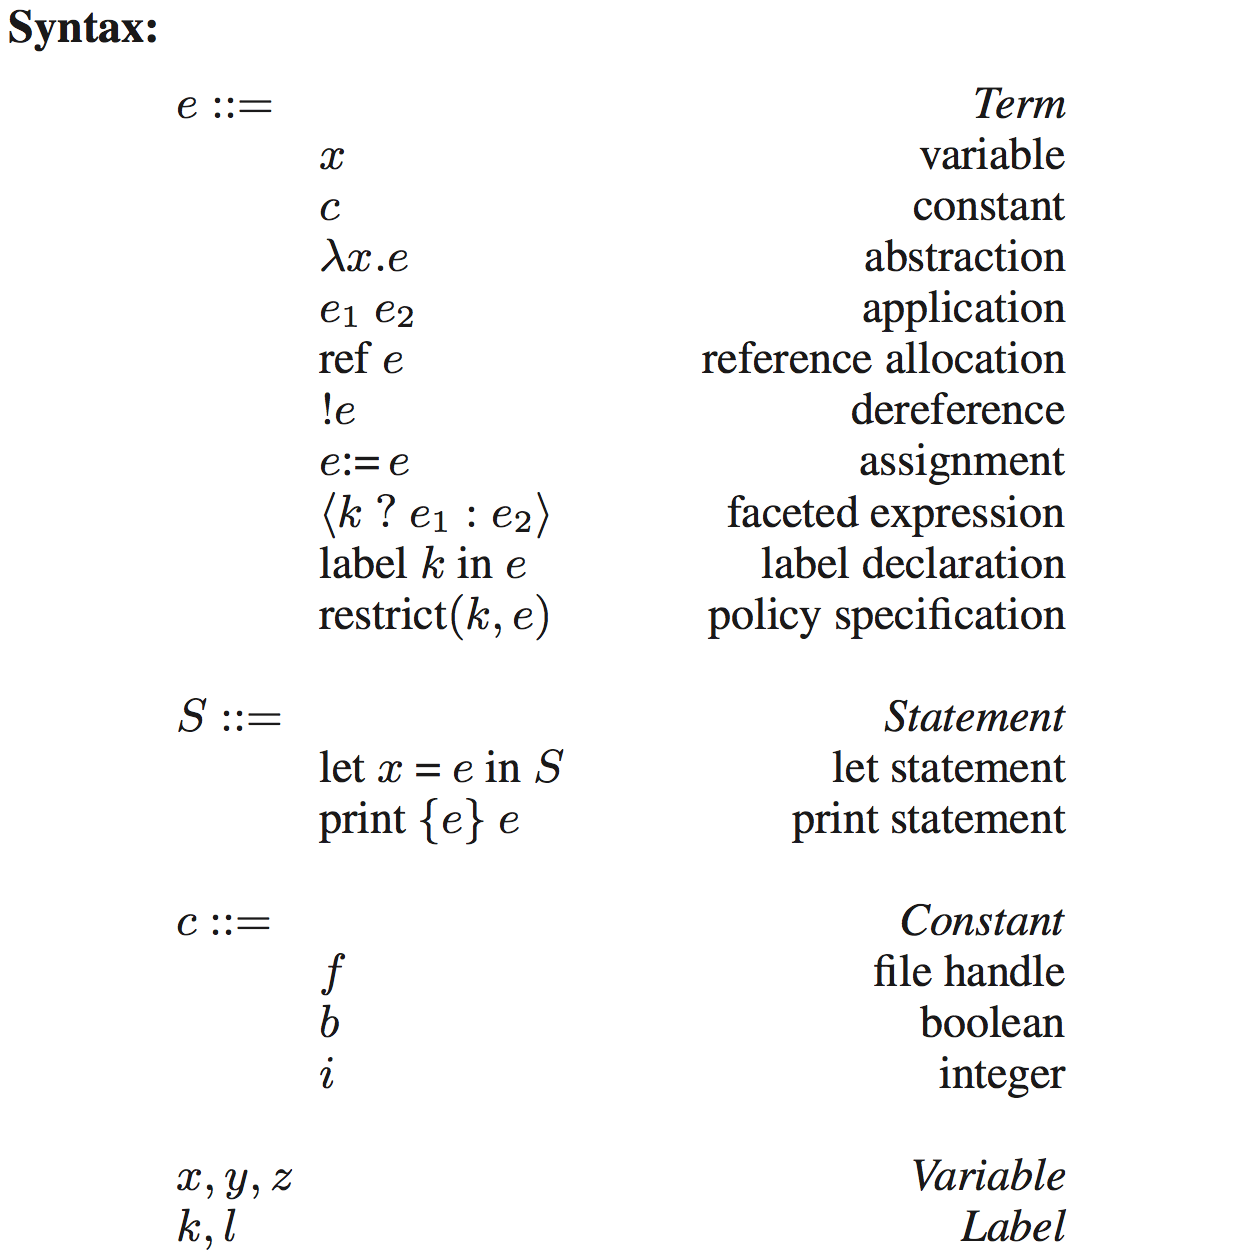
\includegraphics[scale=0.25, frame]{images/lambdaJeeves.png}
	\caption{The $\lambda^{jeeves}$ source language~\cite{FacetedJeeves}}
	\label{fig:lambdaJeeves}
\end{figure}

\begin{figure}
	\centering
	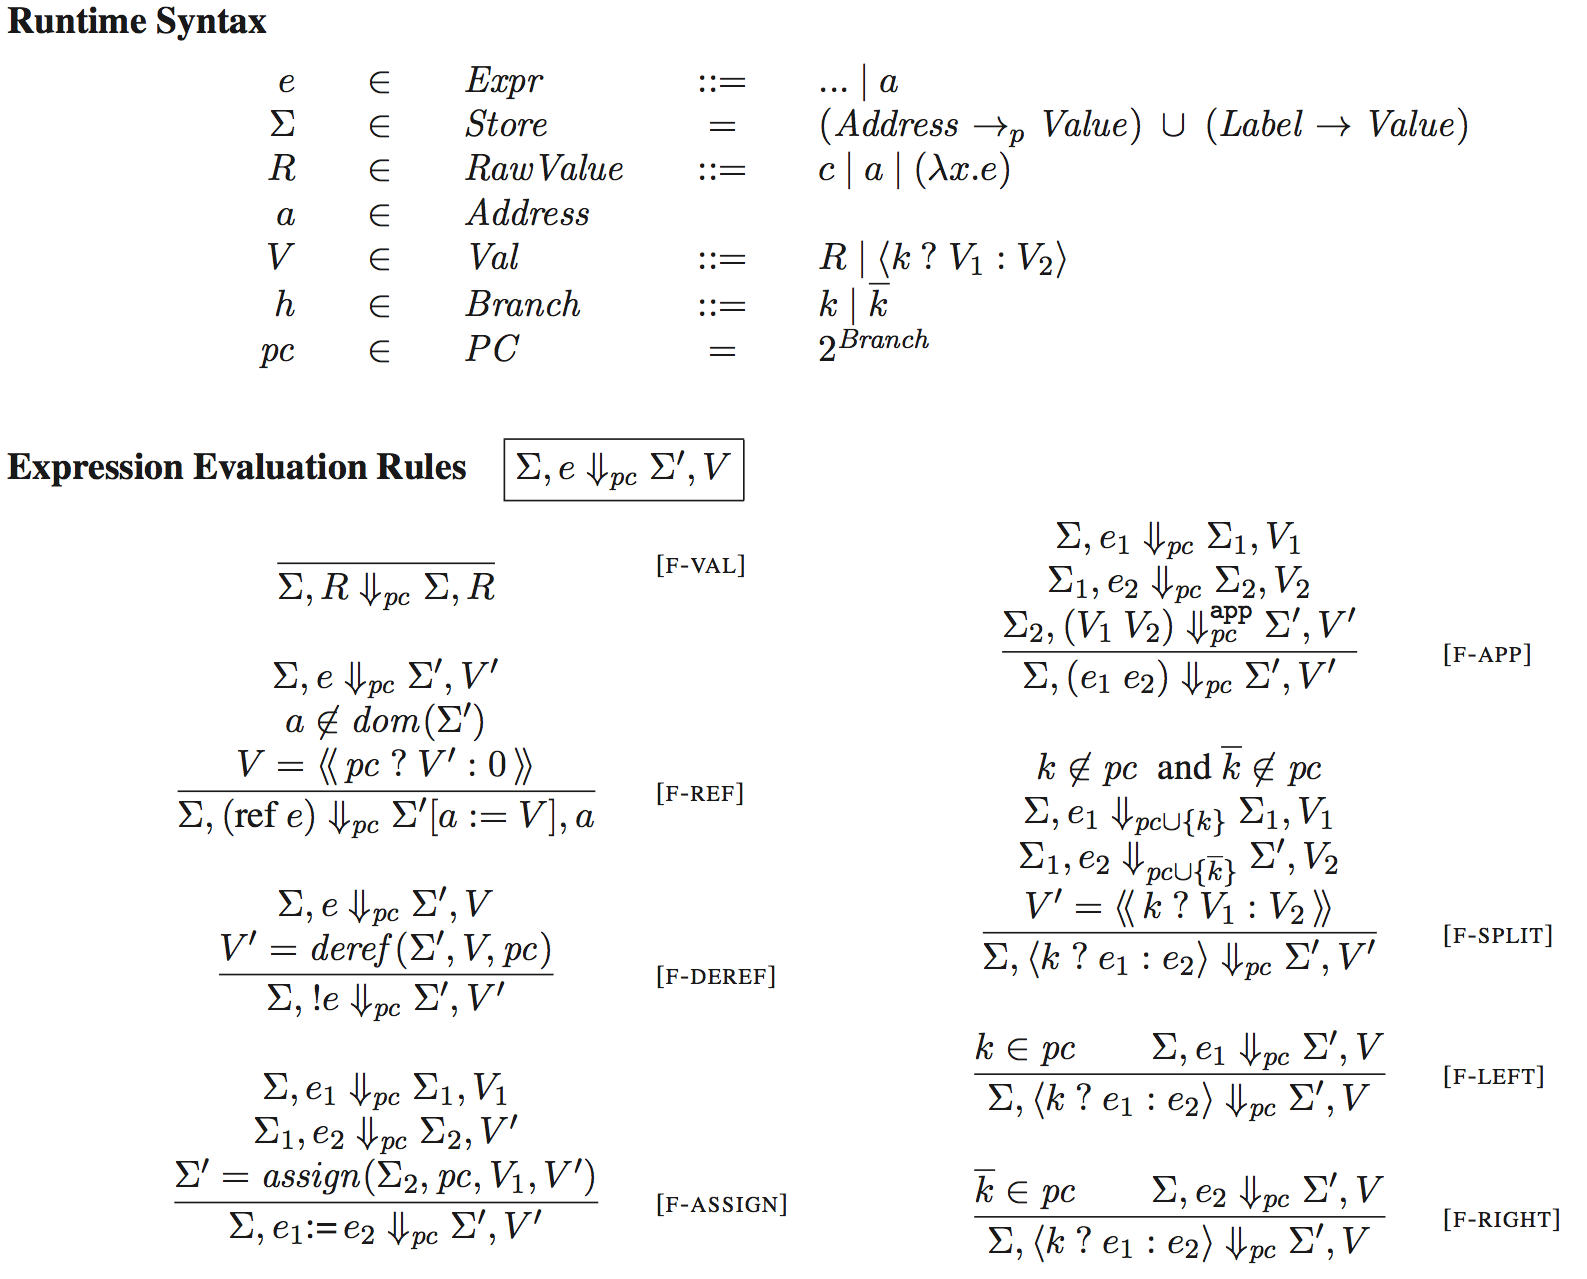
\includegraphics[scale=0.25, frame]{images/facetEval.png}
	\caption{Faceted evaluation semantics~\cite{FacetedJeeves}}
	\label{fig:facetEval}
\end{figure}

In Figure~\ref{fig:fif}, the [F-IF-SPLIT] rule defines how a conditional statement
is handled for faceted values. Figure~\ref{fig:implicit flow} shows how such an
expression would look like in Javascript and it also helps helps us understand
how faceted evaluation would prevent a potential implicit flow. Since the control
flow is being influenced by a faceted value, the behavior of the program under both
facets is evaluated. So, for observers that are allowed to view values with principal
$h$, \texttt{val > 0} would evaluate to true and \texttt{v1} would be equal to 24.
On the other hand, for the public observers, \texttt{val > 0} would evaluate to
false and \texttt{v1} is not assigned any value. The final return value would then
become \texttt{<h?24:undefined>}. Note, if we there was an initial assignment to
\texttt{v1}, then that would be the public facet of the return value instead of
\textit{undefined}.

\begin{figure}
	\centering
	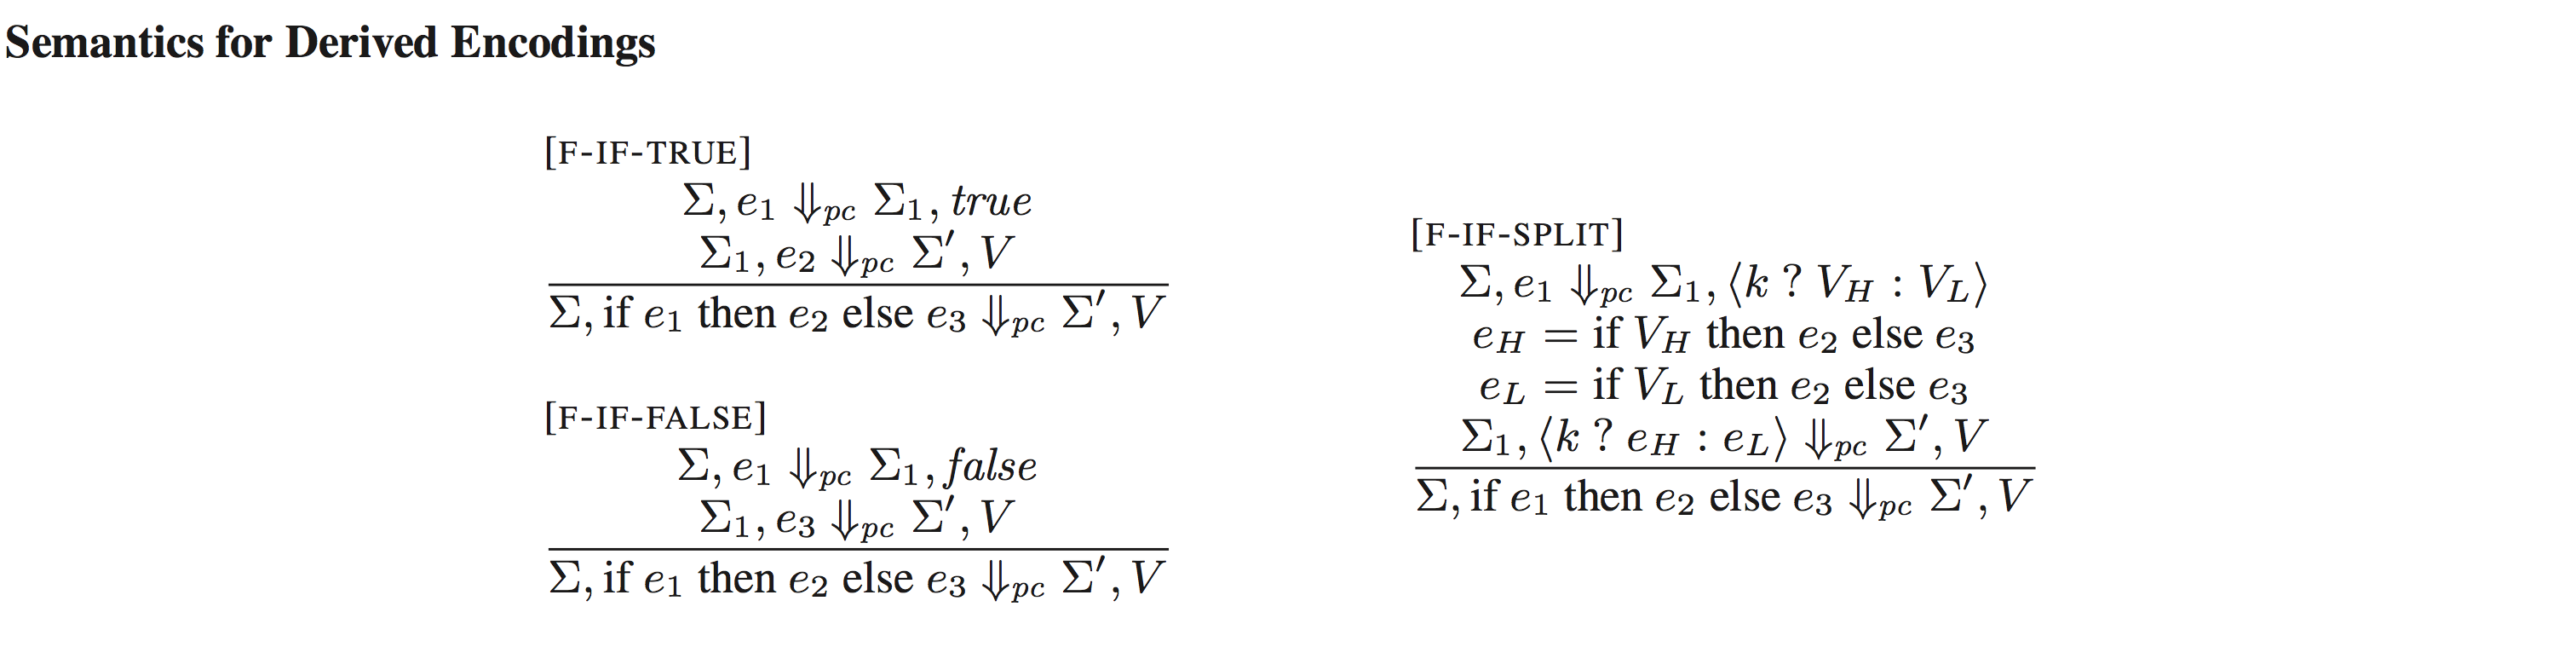
\includegraphics[scale=0.275, frame]{images/fif.png}
	\caption{Semantics of Derived Encodings~\cite{FacetedJeeves}}
	\label{fig:fif}
\end{figure}

\begin{figure}
	\begin{lstlisting}[language=javascript,frame=single, breaklines=true,basicstyle=\footnotesize\ttfamily, numbers=left, extendedchars=true, tabsize=2]
function f(val) {
  var v1;
  if (val > 0) {
    v1 = val - 1;
  }
  return v1;
}
var f1 = <h?25:0>;
f(f1);
\end{lstlisting}
\caption{Faceted Evaluation of a potential implicit flow}
\label{fig:implicit flow}
\end{figure}

The faceted evaluation semantics of Jeeves gives it a few desirable properties;
the \textbf{projection property} which states that a single execution with faceted
values can be projected onto multiple different executions without faceted values,
the termination-insensitive noninterference (the projection property helps to prove
this), and termination-insensitive policy compliance which states that data is revealed
to an external observer only if it is allowed by the policy specified in the program.

\subsection{The Jacqueline Framework}
Yang et al~\cite{Jacqueline} demonstrate the practical feasibility of the policy
agnostic programming paradigm for database-backed server-side applications.
They introduce Jacqueline, an MVC framework with an aim to provide a platform to
easily implement information flow security in server side applications. Figure~\ref{fig:DRS}
shows a snippet of a ``Model'' definition in Jacqueline, how a sensitive value is
defined, and what a policy looks like. Here, \texttt{document\_name} is the field
we are marking as sensitive by using the annotation \texttt{@label\_for}. The method
\texttt{jeeves\_restrict\_documentlabel} defines the policy which as you can see
is a boolean function while the method \texttt{jeeves\_get\_private\_document\_name}
defines the public facet of the sensitive value. Once the policy for a sensitive
variable is defined, the programmer need not worry about where or how they are
using this value, the Jeeves runtime will take care of any potential leaks and the
policy is only resolved when the value is going out to an output context like the
web browser.

\begin{figure}
\begin{lstlisting}[language=Python, frame=single, breaklines=true, keywordstyle=\color{keywords}, stringstyle=\color{red}, identifierstyle=\color{darkgray}, procnamekeys={def,class}, basicstyle=\footnotesize\ttfamily, numbers=left, extendedchars=true, tabsize=2]
class Document(JacquelineModel):
    document_name = models.CharField(max_length = 128)
    description = models.CharField(max_length = 512)
    last_accessed_by = ForeignKey(UserProfile, on_delete=models.CASCADE)
    department = ForeignKey(Department, on_delete=models.CASCADE)
    classification = models.IntegerField(default=Levels.TOP_SECRET)
    project = ForeignKey(Project, on_delete=models.CASCADE)
    filedata = models.FileField(upload_to='rep/')

    @staticmethod
    def jeeves_get_private_document_name(document):
        return "[redacted]"

    @staticmethod
    @label_for('document_name')
    @jeeves
    def jeeves_restrict_documentlabel(document, ctxt):
        return document.classification <= ctxt.clearance and document.department == ctxt.department
\end{lstlisting}
\caption{Model definition in the Jacqueline framework}
\label{fig:DRS}
\end{figure}

As seen in the example above, the Jeeves runtime in the Jacqueline framework took
care of information flow control and resolved the policy for sensitive data only
when going out to the browser. But, once data is on the browser, the concept of
facets is lost but we may want to further protect our data against exfiltration
attacks. This is where our solution would help by persisting faceted values and
policies associated with them on the client-side.

\section{Related Work}
Austin and Flanagan's~\cite{Faceted} original work showed the benefits of
faceted values for dynamic information flow control by giving an example of how
it could help reduce the power of an XSS attack. Rajani et al~\cite{eventDOMIFC}
implement information flow controls for event handling and the DOM API which is
based on work done by Bichhawat et al~\cite{webkitIFC} in which they build information
flow controls into the WebKit Javascript engine. The drawback of both these approaches
is that when an information flow control is violated, the execution is halted which
may not be desirable for dynamic web pages.

Koskela et al~\cite{SecuringWebContent} present an interesting approach to browser
security by presenting an actor based approach where the various content providers
(actors) that make up a web page are accountable for the content they send. They
confine each actor within a \texttt{<div>} tag and based on their track record,
the user/browser can decide how much restriction to enforce on a particular \texttt{<div>}
node.

Policy agnostic programming along with faceted values provides a very flexible
approach (which is desirable on the client-side) to information flow control while
still providing non-interference guarantees. We discuss more about our solution
in Chapter~\ref{chap:solution} along with a demonstration of how it would help
protect browser content.
